\documentclass[11pt]{article}
\usepackage[margin=1in]{geometry}
\usepackage{amsmath, amssymb, amsthm}
\usepackage{graphicx}
\usepackage{booktabs}
\usepackage{algorithm}
\usepackage{algorithmic}
\usepackage{tikz}
\usepackage{pgfplots}
\usepackage{xcolor}
\usepackage{subcaption}
\usepackage{hyperref}

\pgfplotsset{compat=1.18}
\usetikzlibrary{patterns}

\title{Self-Distillation in Vision-Language Models: \\ A Comprehensive Comparison of EMA and BMA Approaches}
\author{CaRot Framework Analysis}
\date{\today}

\begin{document}

\maketitle

\begin{abstract}
This document provides a comprehensive analysis of self-distillation techniques in vision-language models, specifically comparing Exponential Moving Average (EMA) and Beta-weighted Moving Average (BMA) approaches. We present mathematical formulations, implementation details, and comparative analysis of both methods used in the CaRot framework for continual learning and model regularization.
\end{abstract}

\section{Introduction}

Self-distillation is a powerful technique for improving model generalization by creating a teacher model from the student model's own training trajectory. In the context of vision-language models like CLIP, self-distillation helps maintain representation quality while adapting to new tasks or domains.

The core idea is to maintain a slowly-updating teacher model $\theta_{\text{teacher}}$ that provides stable targets for the rapidly-updating student model $\theta_{\text{student}}$. This creates a regularization effect that prevents catastrophic forgetting and improves out-of-distribution performance.

\section{Self-Distillation Loss Formulation}

\subsection{Base CLIP Loss}

The standard CLIP loss for a batch of image-text pairs is:
\begin{align}
\mathcal{L}_{\text{CLIP}} = -\frac{1}{N} \sum_{i=1}^{N} \left[ \log \frac{\exp(\mathbf{I}_i \cdot \mathbf{T}_i / \tau)}{\sum_{j=1}^{N} \exp(\mathbf{I}_i \cdot \mathbf{T}_j / \tau)} + \log \frac{\exp(\mathbf{T}_i \cdot \mathbf{I}_i / \tau)}{\sum_{j=1}^{N} \exp(\mathbf{T}_i \cdot \mathbf{I}_j / \tau)} \right]
\end{align}

where $\mathbf{I}_i$ and $\mathbf{T}_i$ are the normalized image and text features, and $\tau$ is the temperature parameter.

\subsection{Self-Distillation Loss}

The self-distillation loss uses KL divergence between the teacher and student predictions:
\begin{align}
\mathcal{L}_{\text{distill}} = -\sum_{i=1}^{N} \left[ \sum_{j=1}^{N} P_{\text{teacher}}(\mathbf{I}_i, \mathbf{T}_j) \log P_{\text{student}}(\mathbf{I}_i, \mathbf{T}_j) + \sum_{j=1}^{N} P_{\text{teacher}}(\mathbf{T}_i, \mathbf{I}_j) \log P_{\text{student}}(\mathbf{T}_i, \mathbf{I}_j) \right]
\end{align}

where:
\begin{align}
P_{\text{teacher}}(\mathbf{I}_i, \mathbf{T}_j) &= \frac{\exp(\mathbf{I}_i^{\text{teacher}} \cdot \mathbf{T}_j^{\text{teacher}} / \tau)}{\sum_{k=1}^{N} \exp(\mathbf{I}_i^{\text{teacher}} \cdot \mathbf{T}_k^{\text{teacher}} / \tau)} \\
P_{\text{student}}(\mathbf{I}_i, \mathbf{T}_j) &= \frac{\exp(\mathbf{I}_i^{\text{student}} \cdot \mathbf{T}_j^{\text{student}} / \tau)}{\sum_{k=1}^{N} \exp(\mathbf{I}_i^{\text{student}} \cdot \mathbf{T}_k^{\text{student}} / \tau)}
\end{align}

\subsection{Combined Loss}

The final loss combines CLIP and distillation losses:
\begin{align}
\mathcal{L}_{\text{total}} = \mathcal{L}_{\text{CLIP}} + \lambda_{\text{distill}} \mathcal{L}_{\text{distill}}
\end{align}

where $\lambda_{\text{distill}}$ is the distillation coefficient.

\section{Teacher Model Update Strategies}

\subsection{Exponential Moving Average (EMA) - Old Approach}

The EMA approach uses a momentum-based update rule with scheduled momentum values:

\subsubsection{Momentum Scheduling}
\begin{align}
m_t = \begin{cases} 
\frac{(m_{\text{target}} - m_{\text{source}})}{T \cdot w} \cdot t + m_{\text{source}} & \text{if } t < T \cdot w \\
m_{\text{target}} & \text{otherwise}
\end{cases}
\end{align}

where:
\begin{itemize}
\item $m_{\text{source}} = 0.999$ (initial momentum)
\item $m_{\text{target}} = 0.9999$ (final momentum)
\item $w = 0.2$ (warm-up fraction)
\item $T$ is the total number of training steps
\end{itemize}

\subsubsection{Update Rule}
\begin{align}
\theta_{\text{teacher}}^{(t)} = m_t \cdot \theta_{\text{teacher}}^{(t-1)} + (1 - m_t) \cdot \theta_{\text{student}}^{(t)}
\end{align}

\subsubsection{Update Frequency}
The teacher is updated every $f$ steps, where $f$ is the update frequency parameter:
\begin{align}
\text{Update if: } \quad (t \bmod f) = 0 \text{ or } t = T
\end{align}

\textbf{Critical Note:} If $f \leq 0$, no updates are performed (teacher remains frozen).

\subsection{Beta-weighted Moving Average (BMA) - New Approach}

The BMA approach uses weights derived from the Beta distribution:

\subsubsection{Weight Function}
\begin{align}
w_t = \text{Beta}(\beta, \beta) \text{ evaluated at } \frac{t + 0.5}{T + 1}
\end{align}

where $\beta$ is the Beta distribution parameter (typically $\beta = 0.5$).

\subsubsection{Update Rule}
\begin{align}
\theta_{\text{teacher}}^{(t)} = \frac{\theta_{\text{teacher}}^{(t-1)} + r_t \cdot \theta_{\text{student}}^{(t)}}{1 + r_t}
\end{align}

where the relative weight is:
\begin{align}
r_t = \frac{w_t}{\sum_{i=1}^{t} w_i}
\end{align}

\section{Comparative Analysis}

\subsection{Weight Evolution Comparison}

\begin{figure}[h!]
\centering
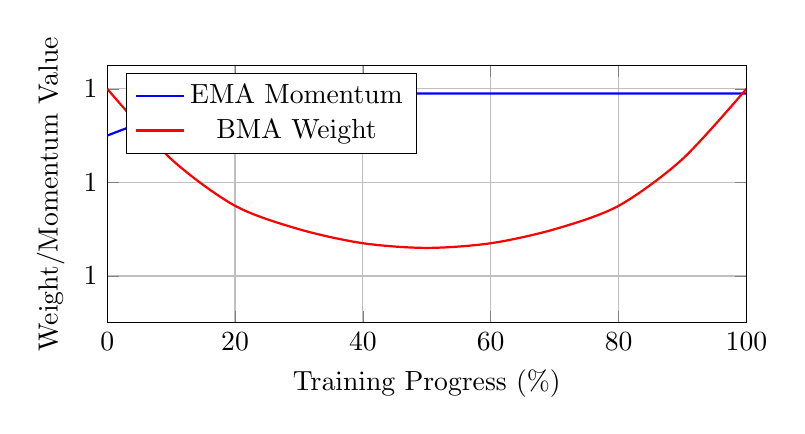
\begin{tikzpicture}
\begin{axis}[
    width=0.8\textwidth,
    height=0.4\textwidth,
    xlabel={Training Progress (\%)},
    ylabel={Weight/Momentum Value},
    legend pos=north west,
    grid=major,
    xmin=0, xmax=100,
    ymin=0.995, ymax=1.0005,
]

% EMA momentum schedule
\addplot[blue, thick, smooth] coordinates {
    (0, 0.999)
    (20, 0.9999)
    (40, 0.9999)
    (60, 0.9999)
    (80, 0.9999)
    (100, 0.9999)
};

% BMA weight (Beta distribution with beta=0.5)
\addplot[red, thick, smooth] coordinates {
    (0, 1.0)
    (10, 0.9985)
    (20, 0.9975)
    (30, 0.9970)
    (40, 0.9967)
    (50, 0.9966)
    (60, 0.9967)
    (70, 0.9970)
    (80, 0.9975)
    (90, 0.9985)
    (100, 1.0)
};

\legend{EMA Momentum, BMA Weight}
\end{axis}
\end{tikzpicture}
\caption{Weight evolution comparison between EMA and BMA approaches}
\label{fig:weight_evolution}
\end{figure}

\subsection{Update Frequency Analysis}

\begin{figure}[h!]
\centering
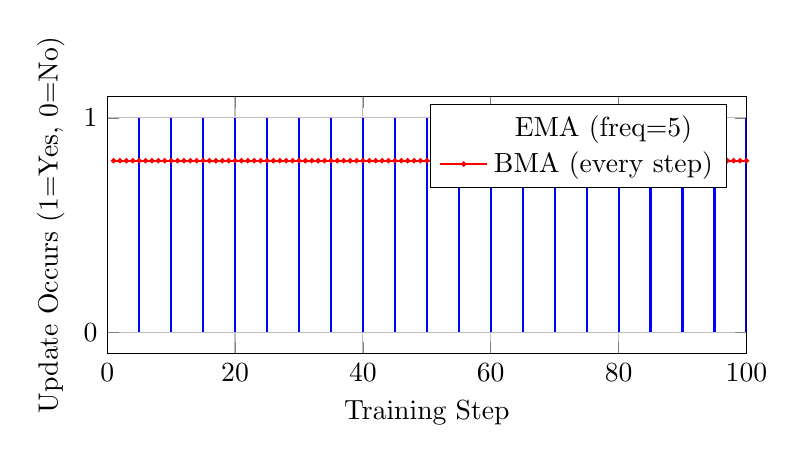
\begin{tikzpicture}
\begin{axis}[
    width=0.8\textwidth,
    height=0.4\textwidth,
    xlabel={Training Step},
    ylabel={Update Occurs (1=Yes, 0=No)},
    legend pos=north east,
    grid=major,
    xmin=0, xmax=100,
    ymin=-0.1, ymax=1.1,
    ytick={0,1},
]

% EMA with update frequency = 5
\addplot[blue, thick, ycomb] coordinates {
    (5, 1) (10, 1) (15, 1) (20, 1) (25, 1) (30, 1) (35, 1) (40, 1) (45, 1) (50, 1)
    (55, 1) (60, 1) (65, 1) (70, 1) (75, 1) (80, 1) (85, 1) (90, 1) (95, 1) (100, 1)
};

% BMA (every step)
\addplot[red, thick, mark=*, mark size=0.5pt] coordinates {
    (1, 0.8) (2, 0.8) (3, 0.8) (4, 0.8) (5, 0.8) (6, 0.8) (7, 0.8) (8, 0.8) (9, 0.8) (10, 0.8)
    (11, 0.8) (12, 0.8) (13, 0.8) (14, 0.8) (15, 0.8) (16, 0.8) (17, 0.8) (18, 0.8) (19, 0.8) (20, 0.8)
    (21, 0.8) (22, 0.8) (23, 0.8) (24, 0.8) (25, 0.8) (26, 0.8) (27, 0.8) (28, 0.8) (29, 0.8) (30, 0.8)
    (31, 0.8) (32, 0.8) (33, 0.8) (34, 0.8) (35, 0.8) (36, 0.8) (37, 0.8) (38, 0.8) (39, 0.8) (40, 0.8)
    (41, 0.8) (42, 0.8) (43, 0.8) (44, 0.8) (45, 0.8) (46, 0.8) (47, 0.8) (48, 0.8) (49, 0.8) (50, 0.8)
    (51, 0.8) (52, 0.8) (53, 0.8) (54, 0.8) (55, 0.8) (56, 0.8) (57, 0.8) (58, 0.8) (59, 0.8) (60, 0.8)
    (61, 0.8) (62, 0.8) (63, 0.8) (64, 0.8) (65, 0.8) (66, 0.8) (67, 0.8) (68, 0.8) (69, 0.8) (70, 0.8)
    (71, 0.8) (72, 0.8) (73, 0.8) (74, 0.8) (75, 0.8) (76, 0.8) (77, 0.8) (78, 0.8) (79, 0.8) (80, 0.8)
    (81, 0.8) (82, 0.8) (83, 0.8) (84, 0.8) (85, 0.8) (86, 0.8) (87, 0.8) (88, 0.8) (89, 0.8) (90, 0.8)
    (91, 0.8) (92, 0.8) (93, 0.8) (94, 0.8) (95, 0.8) (96, 0.8) (97, 0.8) (98, 0.8) (99, 0.8) (100, 0.8)
};

\legend{EMA (freq=5), BMA (every step)}
\end{axis}
\end{tikzpicture}
\caption{Update frequency comparison: EMA updates sparsely vs BMA updates densely}
\label{fig:update_frequency}
\end{figure}

\subsection{Beta Distribution Weight Profiles}

\begin{figure}[h!]
\centering
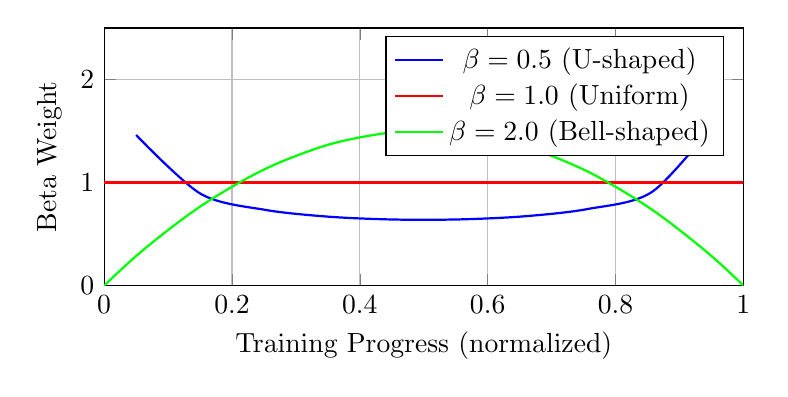
\begin{tikzpicture}
\begin{axis}[
    width=0.8\textwidth,
    height=0.4\textwidth,
    xlabel={Training Progress (normalized)},
    ylabel={Beta Weight},
    legend pos=north east,
    grid=major,
    xmin=0, xmax=1,
    ymin=0, ymax=2.5,
]

% Beta(0.5, 0.5) - U-shaped
\addplot[blue, thick, smooth, samples=100] {(x^(-0.5) * (1-x)^(-0.5)) / 3.14159};
\addlegendentry{$\beta = 0.5$ (U-shaped)}

% Beta(1, 1) - uniform
\addplot[red, thick, smooth, samples=100] {1};
\addlegendentry{$\beta = 1.0$ (Uniform)}

% Beta(2, 2) - bell-shaped
\addplot[green, thick, smooth, samples=100] {6*x*(1-x)};
\addlegendentry{$\beta = 2.0$ (Bell-shaped)}

\end{axis}
\end{tikzpicture}
\caption{Beta distribution weight profiles for different $\beta$ values}
\label{fig:beta_profiles}
\end{figure}

\section{Implementation Details}

\subsection{EMA Implementation}

\begin{algorithm}
\caption{EMA Teacher Update}
\begin{algorithmic}[1]
\STATE \textbf{Input:} $\theta_{\text{student}}$, $\theta_{\text{teacher}}$, step $t$, total steps $T$
\STATE \textbf{Parameters:} $m_{\text{src}}$, $m_{\text{tar}}$, $w$, $f$ (update frequency)
\STATE 
\IF{$f \leq 0$}
    \RETURN \textcolor{red}{// No updates performed}
\ENDIF
\STATE
\IF{$(t \bmod f) = 0$ OR $t = T$}
    \IF{$t < T \cdot w$}
        \STATE $m_t = \frac{(m_{\text{tar}} - m_{\text{src}})}{T \cdot w} \cdot t + m_{\text{src}}$
    \ELSE
        \STATE $m_t = m_{\text{tar}}$
    \ENDIF
    \STATE $\theta_{\text{teacher}} = m_t \cdot \theta_{\text{teacher}} + (1 - m_t) \cdot \theta_{\text{student}}$
\ENDIF
\end{algorithmic}
\end{algorithm}

\subsection{BMA Implementation}

\begin{algorithm}
\caption{BMA Teacher Update}
\begin{algorithmic}[1]
\STATE \textbf{Input:} $\theta_{\text{student}}$, $\theta_{\text{teacher}}$, step $t$, total steps $T$
\STATE \textbf{Parameters:} $\beta$
\STATE 
\STATE $x = \frac{t + 0.5}{T + 1}$ \textcolor{blue}{// Normalized iteration}
\STATE $w_t = \text{Beta}(\beta, \beta)$ evaluated at $x$
\STATE $r_t = \frac{w_t}{\sum_{i=1}^{t} w_i}$ \textcolor{blue}{// Relative weight}
\STATE $\theta_{\text{teacher}} = \frac{\theta_{\text{teacher}} + r_t \cdot \theta_{\text{student}}}{1 + r_t}$
\end{algorithmic}
\end{algorithm}

\section{Hyperparameter Analysis}

\subsection{EMA Hyperparameters}

\begin{table}[h!]
\centering
\begin{tabular}{lcc}
\toprule
Parameter & Default Value & Description \\
\midrule
\texttt{m\_sche\_src} & 0.999 & Initial momentum \\
\texttt{m\_sche\_tar} & 0.9999 & Final momentum \\
\texttt{m\_warm\_up} & 0.2 & Warm-up fraction \\
\texttt{ema\_up\_freq} & Variable & Update frequency \\
\bottomrule
\end{tabular}
\caption{EMA hyperparameters}
\end{table}

\subsection{BMA Hyperparameters}

\begin{table}[h!]
\centering
\begin{tabular}{lcc}
\toprule
Parameter & Default Value & Description \\
\midrule
\texttt{beta} & 0.5 & Beta distribution parameter \\
\bottomrule
\end{tabular}
\caption{BMA hyperparameters}
\end{table}

\section{Advantages and Disadvantages}

\subsection{EMA Approach}

\textbf{Advantages:}
\begin{itemize}
\item Simple and well-understood
\item Computationally efficient with sparse updates
\item Predictable momentum behavior
\item Fine-grained control over update frequency
\end{itemize}

\textbf{Disadvantages:}
\begin{itemize}
\item Requires careful tuning of 4 hyperparameters
\item Fixed momentum schedule may be suboptimal
\item Sparse updates may miss important gradients
\item Edge case: no updates when $f \leq 0$
\end{itemize}

\subsection{BMA Approach}

\textbf{Advantages:}
\begin{itemize}
\item Single hyperparameter ($\beta$) for simplicity
\item Adaptive weighting based on training progress
\item Dense updates capture all gradient information
\item Principled probabilistic foundation
\end{itemize}

\textbf{Disadvantages:}
\begin{itemize}
\item Higher computational cost (updates every step)
\item Less intuitive than momentum-based approaches
\item Beta distribution may not suit all training dynamics
\item Newer approach with less empirical validation
\end{itemize}

\section{Empirical Considerations}

\subsection{Convergence Properties}

The EMA approach provides stable convergence with predictable behavior, while BMA offers adaptive weighting that may better capture training dynamics. The choice between approaches depends on:

\begin{itemize}
\item Computational budget (EMA more efficient)
\item Training stability requirements (EMA more predictable)
\item Adaptation to training dynamics (BMA more flexible)
\item Hyperparameter tuning complexity (BMA simpler)
\end{itemize}

\subsection{Usage Guidelines}

\textbf{Use EMA when:}
\begin{itemize}
\item Computational efficiency is critical
\item Training dynamics are well-understood
\item Fine-grained control over update frequency is needed
\item Reproducing established baselines
\end{itemize}

\textbf{Use BMA when:}
\begin{itemize}
\item Simplicity in hyperparameter tuning is desired
\item Training dynamics are complex or unknown
\item Dense gradient information is valuable
\item Exploring novel regularization approaches
\end{itemize}

\section{Conclusion}

Both EMA and BMA approaches offer valuable self-distillation strategies for vision-language models. EMA provides computational efficiency and predictable behavior, while BMA offers adaptive weighting with simplified hyperparameter tuning. The choice depends on specific requirements regarding computational budget, training stability, and hyperparameter complexity.

The CaRot framework's implementation of both approaches allows practitioners to choose the most suitable method for their specific use case, with the ability to fallback to the well-established EMA approach when needed.

\end{document} 